\subsection{线性表的顺序存储}
\begin{frame}\ft{\subsecname}
\begin{dingyi}[顺序存储]
把结点按逻辑顺序依次存放在一组地址连续的存储单元里, 
以这种方式存储的线性表简称顺序表( Sequence List)。
\end{dingyi}

\pause 
\textcolor{acolor5}{特点}
\begin{itemize}
\item
逻辑顺序与物理顺序一致;
\item
数据元素之间的关系是以元素在计算机内”物理位置相邻“来体现的. 
\end{itemize}
\end{frame}

\begin{frame}\ft{\subsecname}
设有非空线性表$(a_1,a_2,\cd,a_n)$,  $l_i$表示$a_i$的存储位置,  $k$为每个元素需占用的存储单元. 
\begin{figure}
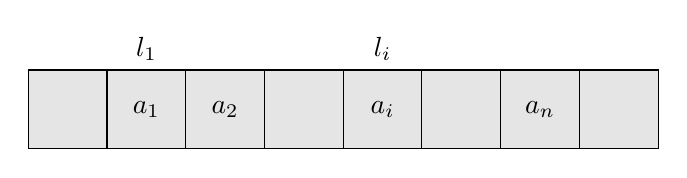
\begin{tikzpicture}
\foreach \i in {1,...,8}
\filldraw[fill=black!10] (\i-1,0)rectangle(\i,1);
\node [] at (0.5,0.5) {$\cd$};
\node [] at (1.5,0.5) {$a_1$}; \node [above] at (1.5,1) {$l_1$}; 
\node [] at (2.5,0.5) {$a_2$};
\node [] at (3.5,0.5) {$\cd$};
\node [] at (4.5,0.5) {$a_i$}; \node [above] at (4.5,1) {$l_i$}; 
\node [] at (5.5,0.5) {$\cd$};
\node [] at (6.5,0.5) {$a_n$};
\node [] at (7.5,0.5) {$\cd$};
\end{tikzpicture}
\caption{线性表的顺序存储}
\end{figure}

%第$i+1$个数据元素的存储位置$Loc(a_{i+1})$和第$i$个数据元素的存储位置$Loc(a_{i})$之间满足
$$
l_{i+1}=l_{i}+k
$$
%其中$l$为线性表每个元素需占用的存储单元. 特别地,  
$$
l_{i}=l_{1}+(i-1)k
$$
\end{frame}

\begin{frame}[fragile]\ft{\subsecname}
\begin{lstlisting}[title=顺序存储的结构代码,language=C,frame=tb,backgroundcolor=\color{red!10}]
#define MAX_SIZE 100
typedef int ElemType;
typedef struct sqlist {
    ElemType data[MAX_SIZE];
    int length;
} SqList;
\end{lstlisting}


%% \begin{itemize}
%% \item 存储空间的起始位置: 数组{\ttfamily elem\_array}, 其存储位置就是存储空间的存储位置
%% \item 线性表的最大存储容量: 数组长度{\ttfamily MAX\_SIZE}
%% \item 线性表的当前长度: {\ttfamily length}
%% \end{itemize}
\end{frame}
%
\begin{frame}\ft{\subsecname}
\begin{zhu}[数据长度与线性表长度的区别]
\begin{itemize}
\item 数组长度是存放线性表存储空间的长度,存储分配后一般不变; 
\item 线性表长度是线性表中数据元素的个数,随着线性表插入和删除操作的进行而发生变化; 
\item 线性表长度总小于等于数组长度。
\end{itemize}
\end{zhu}
\end{frame}
%
\begin{frame}\ft{顺序表的基本操作}
\begin{itemize}
\item
初始化
\item
赋值
\item
查找
\item
修改
\item
插入
\item
删除
\item
求长度
\item
$\cd$
\end{itemize}•
\end{frame}
%

\begin{frame}[fragile]\ft{顺序表的基本操作}
\lstinputlisting
[title=SqList.h,language=C,linerange={1-9}]
{Chapters/Ch02/Code/SqList/SqList.h}
\end{frame}
%
\begin{frame}[fragile]\ft{顺序表的基本操作:初始化}
\lstinputlisting
[
title=SqListInit.c,
language=C,
linerange={3-15},
numbers=left,
firstnumber=auto,
]
{Chapters/Ch02/Code/SqList/SqListInit.c}
\end{frame}

\begin{frame}[fragile]\ft{顺序表的基本操作:插入结点}
\textcolor{acolor5}{目标:}
在$L=(a_1,\cd,a_{i-1},\textcolor{acolor3}{a_i},a_{i+1},\cd,a_n)$中的第$i$个位置上插入新结点$e$,  使其成为
$$
L=(a_1,\cd,a_{i-1},e,a_i,a_{i+1},\cd,a_n)
$$
\end{frame}

\begin{frame}[fragile]\ft{顺序表的基本操作:插入结点} 
\textcolor{acolor5}{实现步骤}
\begin{itemize}
\item
如果插入位置不合理,抛出异常;
\item
如果线性表长度大于等于数组长度,抛出异常或动态增加容量;
\item
从最后一个元素开始向前遍历到第$i$个位置,分别将它们向后移动一个位置;
\item
将元素$e$填入位置$i$处;
\item
线性表长度加$1$。
\end{itemize}

\end{frame}

\begin{frame}[fragile]\ft{顺序表的基本操作:插入结点} 
\lstinputlisting
[
title=SqListInsert.c,
language=C,
linerange={3-10},
numbers=left,
firstnumber=auto,
]
{Chapters/Ch02/Code/SqList/SqListInsert.c}
\end{frame}

\begin{frame}[fragile]\ft{顺序表的基本操作:插入结点} 
\lstinputlisting
[
title=SqListInsert.c,
language=C,
linerange={12-18},
numbers=left,
firstnumber=9,
]
{Chapters/Ch02/Code/SqList/SqListInsert.c}
\end{frame}

\begin{frame}\ft{顺序表的基本操作:插入结点} 
在$L$的第$i$个元素之前插入新结点,  其时间主要耗费在结点的移动上. 因此,  可用结点的移动来估计算法的时间复杂度.  \vspace{0.1in}

设在$L$的第$i$个元素之前插入结点的概率为$p_i$. 不失一般性,  设各位置插入等概率,  则$p_i=\frac1{n+1}$,  而插入时移动结点的次数为$n-i+1$,  故总的平均移动次数为
$$
E_{insert}=\sum_{i=1}^n p_i (n-i+1)=\frac n2.
$$ 

这表明,  在顺序表上做插入运算,  平均要移动表上一半的结点. 当表长$n$较大时,  算法效率相当低. 因此算法的平均时间复杂度为$O(n)$. 
\end{frame}

\begin{frame}\ft{顺序表的基本操作:删除结点}
\textcolor{acolor5}{目标}
在
$$
L=(a_1,\cd,a_{i-1},\textcolor{acolor3}{a_i},a_{i+1},\cd,a_n)
$$
中删除结点$a_i$,  使其成为 
$$
L=(a_1,\cd,a_{i-1},a_{i+1},\cd,a_n)
$$
\end{frame}

\begin{frame}\ft{顺序表的基本操作:删除结点}  
\textcolor{acolor5}{实现步骤}
\begin{itemize}
\item
若删除位置不合理,抛出异常;
\item
取出删除元素;
\item
从删除元素的位置开始遍历到最后一个元素的位置,分别将它们向前移动一个位置;
\item
表长减$1$.
\end{itemize}
\end{frame}


\begin{frame}[fragile]\ft{顺序表的基本操作:删除结点}
\lstinputlisting
[
title=SqListDelete.c,
language=C,
linerange={3-10},
numbers=left,
firstnumber=auto,
]
{Chapters/Ch02/Code/SqList/SqListDelete.c}
\end{frame}

\begin{frame}[fragile]\ft{顺序表的基本操作:删除结点}
\lstinputlisting
[
title=SqListDelete.c,
language=C,
linerange={11-22},
numbers=left,
firstnumber=9,
]
{Chapters/Ch02/Code/SqList/SqListDelete.c}
\end{frame}
%
%
\begin{frame}\ft{顺序表的基本操作:删除结点} 
删除$L$的第$i$个元素,  其时间主要耗费在表中结点的移动操作上. 因此,  可用结点的移动来估计算法的时间复杂度. \vspace{0.1in}

设在$L$中删除第$i$个元素的概率为$p_i$,  不失一般性,  设各个位置插入等概率,  则$p_i=\frac1{n}$,  而插入时移动结点的次数为$n-i$,  故总的平均移动次数为
$$
E_{delete}=\sum_{i=1}^n p_i (n-i)=\frac {n-1}2.
$$

这表明,  在顺序表上做删除运算,  平均要移动表上一半的结点. 当表长$n$较大时,  算法效率相当低. 因此算法的平均时间复杂度为$O(n)$. 
\end{frame}

\begin{frame}\ft{顺序表的基本操作:查找、定位删除}
\textcolor{acolor5}{目标:}
在$L=(a_1,a_2,\cd,a_n)$中删除值为$x$的第一个结点. 

\pause 
\textcolor{acolor5}{实现步骤:}
\begin{enumerate}
\item 
在$L$中查找值为$x$的第一个元素;
\item 
将从找到的位置至最后一个结点依次向前移动一个位置;
\item 
线性表长度减$1$。 
\end{enumerate}
\end{frame}


\begin{frame}[fragile]\ft{顺序表的基本操作:查找、定位删除}
\lstinputlisting
[
title=SqListLocateDelete.c,
language=C,
linerange={3-6},
numbers=left,
firstnumber=auto,
]
{Chapters/Ch02/Code/SqList/SqListLocateDelete.c}
\end{frame}

\begin{frame}[fragile]\ft{顺序表的基本操作:查找、定位删除}
\lstinputlisting
[
title=SqListLocateDelete.c,
language=C,
linerange={7-17},
numbers=left,
firstnumber=5,
]
{Chapters/Ch02/Code/SqList/SqListLocateDelete.c}
\end{frame}

\begin{frame}[fragile]\ft{顺序表的基本操作:查找、定位删除}
\lstinputlisting
[
title=SqListLocateDelete.c,
language=C,
linerange={19-29},
numbers=left,
firstnumber=16,
]
{Chapters/Ch02/Code/SqList/SqListLocateDelete.c}
\end{frame}

\begin{frame}\ft{顺序表的基本操作:查找、定位删除}
时间主要耗费在数据元素的比较和移动操作上. \vspace{0.1in}

设在$L$中删除数据元素的概率为$p_i$,  不失一般性,  设各个位置等概率,  则$p_i=\frac1{n}$. 
\begin{itemize}
\item 比较的平均次数为:
$$
E_{compare} = \sum_{i=1}^n p_i i= \frac{n+1}2
$$
\item 删除时的平均移动次数为
$$
E_{delete} =\sum_{i=1}^n p_i (n-i)=\frac {n-1}2.
$$\
\end{itemize}
平均时间复杂度为
\[
E_{compare}+E_{delete}=n
\]

\end{frame}


\begin{frame}\ft{顺序表的优缺点}
\textcolor{acolor5}{优点}
\begin{itemize}
\item 无须为表示表中元素之间的逻辑关系而增加额外的存储空间
\item 可以快速地存取表中任一位置的元素
\end{itemize}
 

\pause

\textcolor{acolor5}{缺点}
\begin{itemize}
\item 插入和删除操作需要移动大量元素
\item 当线性表变化较大时,难以确定存储空间的容量
\item 造成存储空间的“碎片”
\end{itemize}


\end{frame}
